\documentclass[12pt]{article}%
\usepackage{amsfonts}

\usepackage[utf8]{inputenc}
\usepackage[spanish]{babel}
\usepackage{booktabs}

\usepackage{fancyhdr}
\usepackage{comment}
\usepackage[a4paper, top=2.5cm, bottom=2.5cm, left=2.2cm, right=2.2cm]%
{geometry}
\usepackage{amsmath}
\usepackage{changepage}
\usepackage{amssymb}
\usepackage{graphicx}%
\setcounter{MaxMatrixCols}{30}

\begin{document}
\textbf{Definición:} El \textit{timespan} para un líder es la cantidad de años comprendida entre el primer discurso y el último discurso en la muestra. Si $year_{min}$ es el año del discurso más temprano y $year_{max}$ es el año del discurso más tardío, entonces $\text{\textit{timespan}}=year_{max}-year_{min}+1.$
	
\section{Resultados para líderes con \textit{timespan}$>=11$}
Esta muestra contiene 97 líderes con \textit{timespan} mayor o igual a 11 años. Se separaron sus discursos en dos grupos:
\begin{itemize}
	\item Grupo 1: Discursos con fecha dentro del intervalo $[year_{min},year_{min}+4].$
	\item Grupo 2: Discursos con fecha dentro del intervalo $[year_{max}-4,year_{max}].$
\end{itemize}

\textbf{Observación:} en realidad 11 años no es la mediana de los \textit{timespans} de los líderes. Un 57,5\% de los líderes tiene un \textit{timespan} menor que 11. La mediana se ubica en 7 años.


\subsection{Rank-sum test de media}
No se observan diferencias significativas en ningún Big Five.
\begin{table}[htpb]
	\centering
	\caption{Resultados Rank-sum test de media entre los Big Five estimados para los Grupo 1 y 2}
	\label{my-label}
	\begin{tabular}{ll}
		\toprule\toprule
		Big Five                & Rank-sum p-value \\
		\midrule
		Extraversión            & 0.5719           \\
		Inestabilidad emocional & 0.8021           \\
		Amabilidad              & 0.2046           \\
		Responsabilidad         & 0.7991           \\
		Apertura al cambio      & 0.6815   \\
		\bottomrule \bottomrule   
	\end{tabular}
\end{table}

\subsection{Test de Kolmogorov-Smirnov}
No se observan diferencias significativas en ningún Big Five.
\begin{table}[htpb]
	\centering
	\caption{Resultados test de Kolmogorov-Smirnov de igual de la distribución entre los Big Five estimados para los Grupo 1 y 2}
	\label{my-label}
	\begin{tabular}{lll}
		\toprule\toprule
		Big Five                & KS p-value & Corrected\\
		\midrule
		Extraversión            & 0.798&0.749          \\
		Inestabilidad emocional & 0.798&0.749\footnote{Se obtiene efectivamente el mismo $p-value$ que en extraversión (¿raro no?)}           \\
		Amabilidad              & 0.196 & 0.155           \\
		Responsabilidad         & 0.561 &    0.497         \\
		Apertura al cambio      & 0.896 & 0.864   \\
		\bottomrule \bottomrule   
	\end{tabular}
\end{table}

\subsection{Histogramas}

\begin{figure}[htpb]
	\centering
	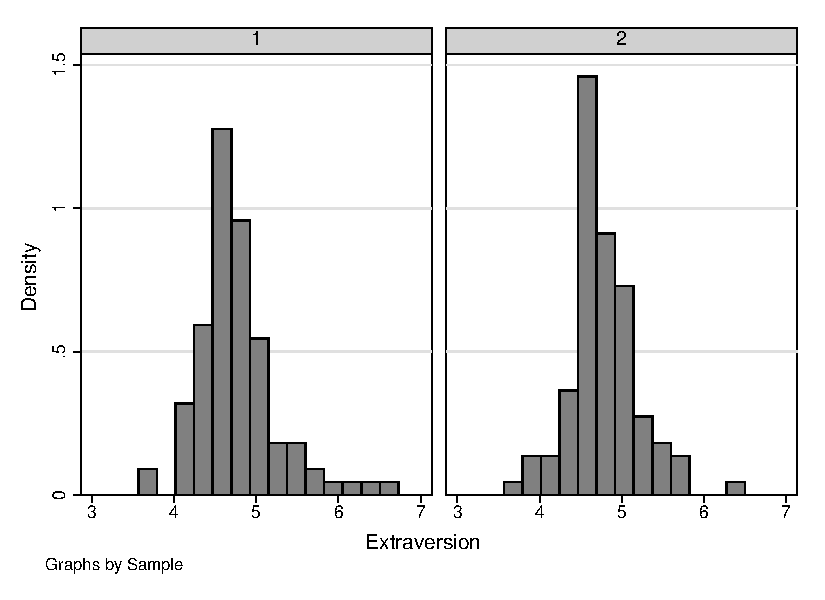
\includegraphics[]{extraversion.pdf}
	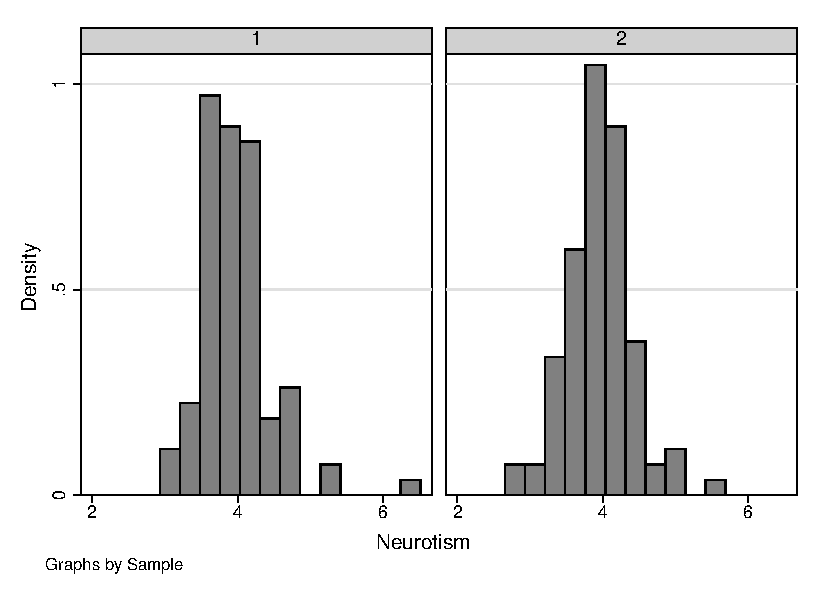
\includegraphics[]{neurotism.pdf}
\end{figure}
\begin{figure}[htpb]
	\centering
	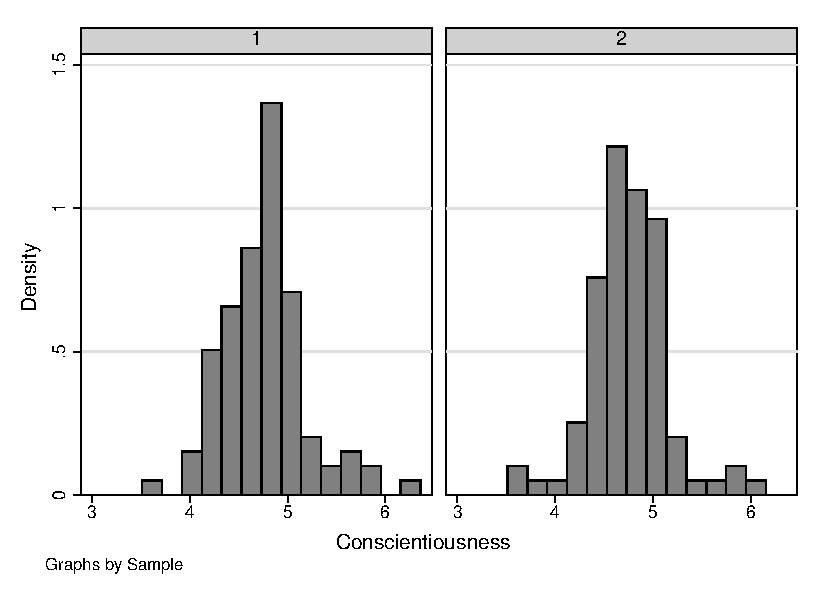
\includegraphics[]{conscientiousness.pdf}
	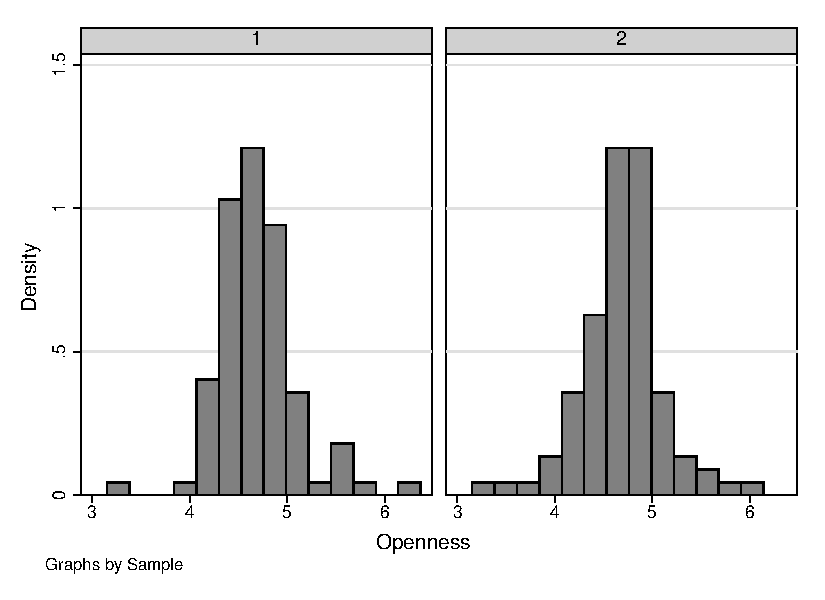
\includegraphics[]{openness.pdf}
\end{figure}
\begin{figure}[htpb]
	\centering
	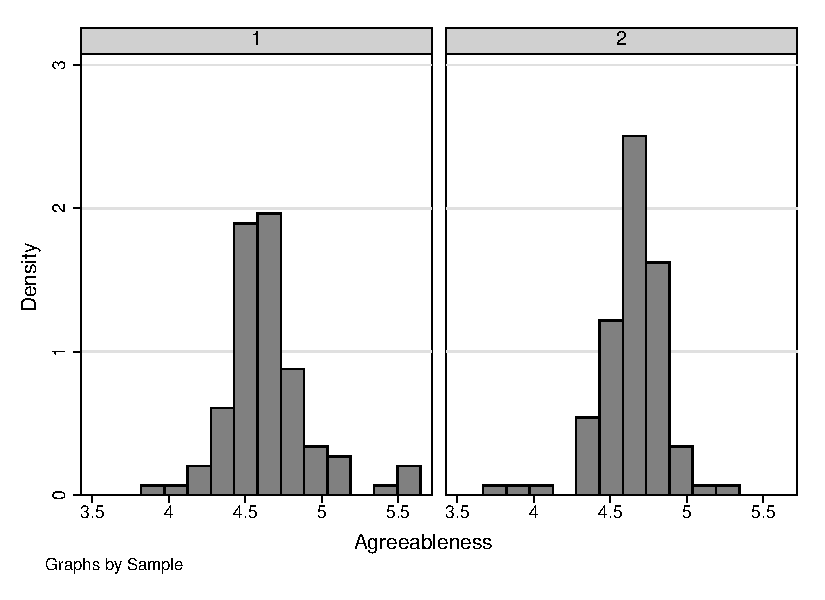
\includegraphics[]{agreeableness.pdf}
\end{figure}
\clearpage
\section{Resultados para líderes con \textit{timespan}$>=22$ (último quintil)}

Esta muestra contiene 45 líderes con \textit{timespan} mayor o igual a 22 años. Tal como en el caso previo, se separaron sus discursos en dos grupos:
\begin{itemize}
	\item Grupo 1: Discursos con fecha dentro del intervalo $[year_{min},year_{min}+4].$
	\item Grupo 2: Discursos con fecha dentro del intervalo $[year_{max}-4,year_{max}].$
\end{itemize}


\subsection{Rank-sum test de media}
No se observan diferencias significativas en ningún Big Five.
\begin{table}[htpb]
	\centering
	\caption{Resultados Rank-sum test de media entre los Big Five estimados para los Grupo 1 y 2}
	\label{my-label}
	\begin{tabular}{ll}
		\toprule\toprule
		Big Five                & Rank-sum p-value \\
		\midrule
		Extraversión            & 0.8370           \\
		Inestabilidad emocional & 0.3618           \\
		Amabilidad              & 0.3576          \\
		Responsabilidad         & 0.8877           \\
		Apertura al cambio      & 0.8244   \\
		\bottomrule \bottomrule   
	\end{tabular}
\end{table}

\subsection{Test de Kolmogorov-Smirnov}
No se observan diferencias significativas en ningún Big Five.
\begin{table}[htpb]
	\centering
	\caption{Resultados test de Kolmogorov-Smirnov de igual de la distribución entre los Big Five estimados para los Grupo 1 y 2}
	\label{my-label}
	\begin{tabular}{lll}
		\toprule\toprule
		Big Five                & KS p-value & Corrected\\
		\midrule
		Extraversión            &  0.944   &  0.915          \\
		Inestabilidad emocional & 0.648   &   0.565         \\
		Amabilidad              & 0.476   &   0.391           \\
		Responsabilidad         & 0.648   &   0.565        \\
		Apertura al cambio      & 0.944   &  0.915   \\
		\bottomrule \bottomrule   
	\end{tabular}
\end{table}

\subsection{Histogramas}
\begin{figure}
	\centering
	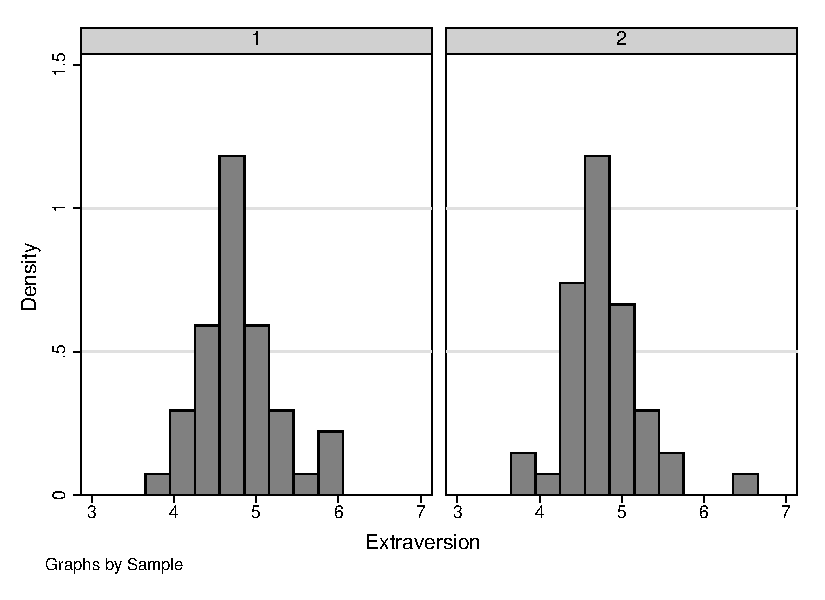
\includegraphics[]{extraversion2.pdf}
	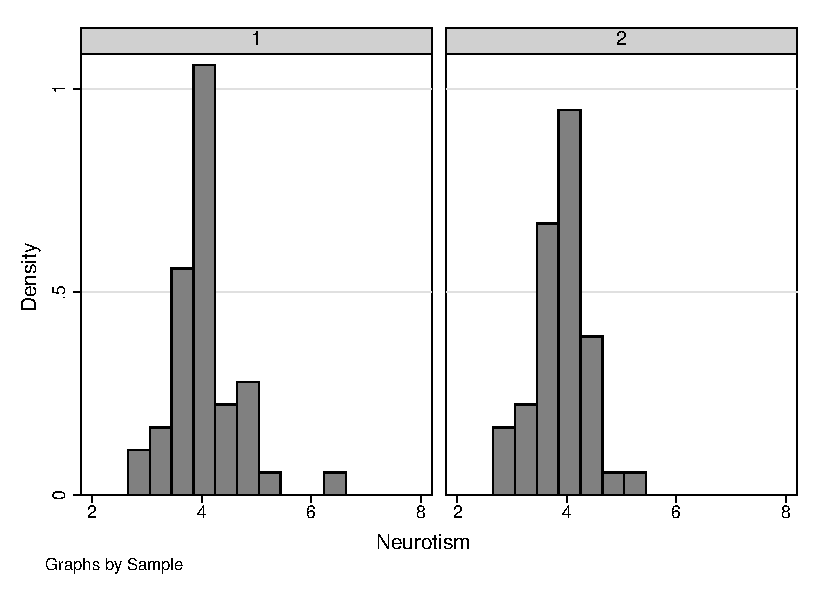
\includegraphics[]{neurotism2.pdf}
\end{figure}
\begin{figure}
	\centering
	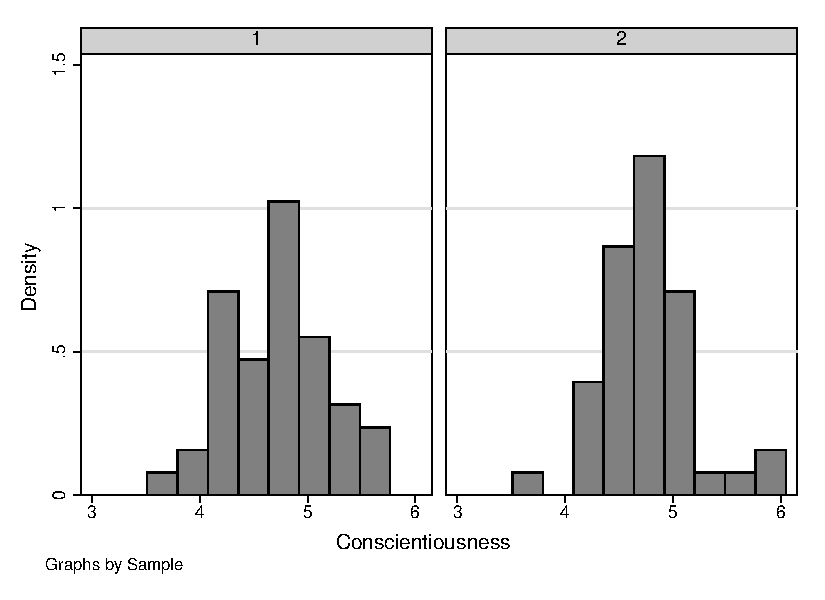
\includegraphics[]{conscientiousness2.pdf}
	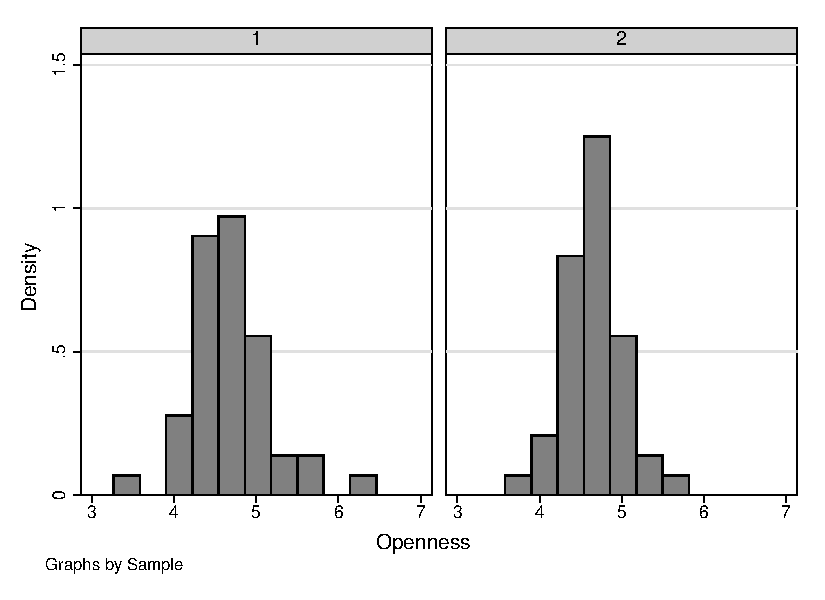
\includegraphics[]{openness2.pdf}
\end{figure}
\begin{figure}
	\centering
	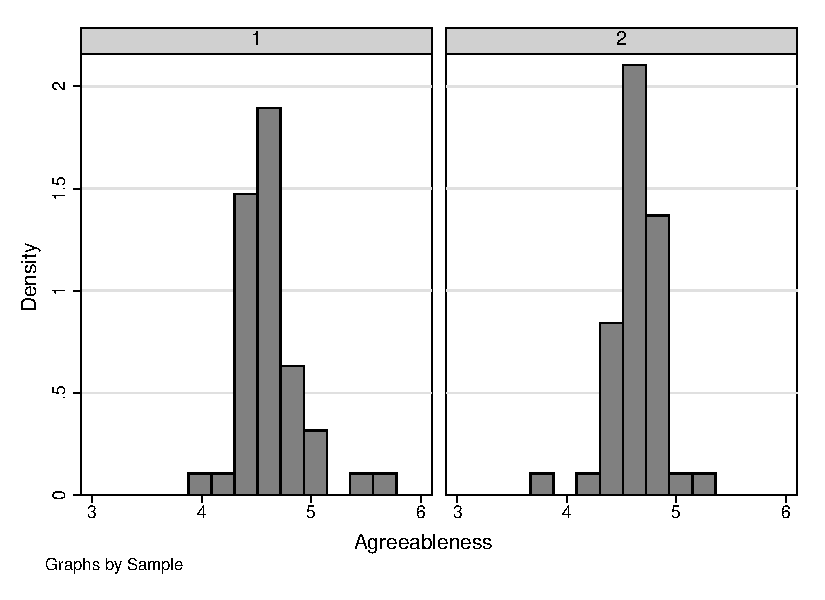
\includegraphics[]{agreeableness2.pdf}
\end{figure}


\end{document}